

\section{Discharge Apparatus}

The design of the \acs{rpnd} apparatus was similar to the coaxial geometry used
by Vasilyak and others in \acs{fiw} studies \cite{Vasilyak1994}. Broadly, it was
comprised of cylindrical inner conductor, surrounded by a dielectric, surrounded
by an outer conductor. In this case, two electrodes and the \acs{rpnd} between
them served as the inner conductor. The dielectric was provided by a glass tube
and an air gap. Finally, the outer conductor was an aluminum shell. This
configuration has the benefit of minimizing the undesired inductance of the
system which could inhibit the propagation of the exciting voltage pulse.
The geometry and its electrical equivalent are sketched in
figure~\ref{fig:appschem}.
\begin{figure}
  \centering
  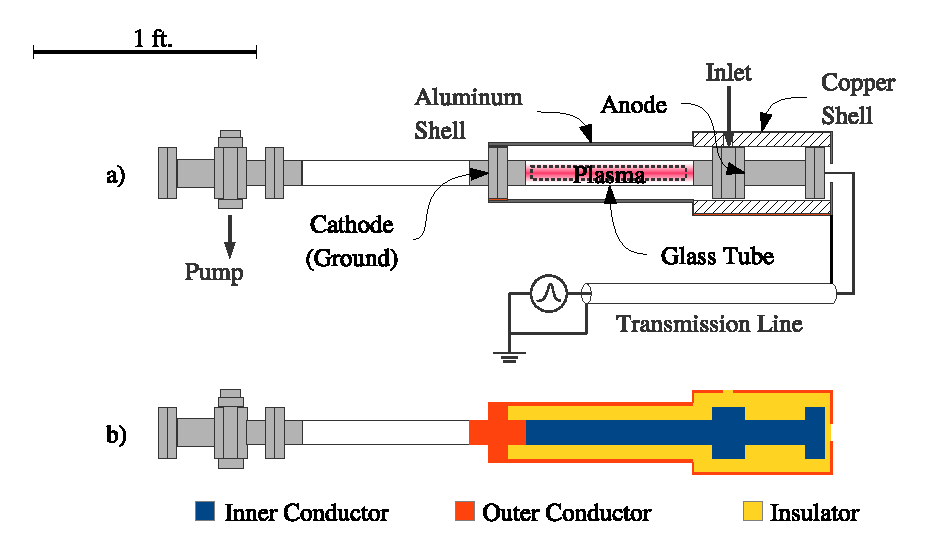
\includegraphics{./chapters/experiment/figures/appschem.eps}
  \caption{Two illustrations of the \acs{rpnd} apparatus. The upper version is
    an annotated sketch of the device, and the bottom version simplifies the
    geometry into its three electrical components.}
  \label{fig:appschem}
\end{figure}
Following from right to left, the inner conductor was composed of a vacuum
window, a Conflat nipple, a double-sided flange tapped for an \textsc{npt}
connection, and the discharge tube containing the plasma.

The tube was composed of borosilicate glass with 2.75 in Conflat flanges on both
ends. The plasma was generated inside the glass tube after it had been evacuated
of air and filled with the desired pressure of helium. The tube had an inner
diameter of 3.3 cm, an outer diameter of 4.0 cm, and a length of 22.9 cm. The
overall length of the tube with the flanges was 30 cm. In the figure shown here,
the right electrode served as the anode, and the left electrode was the cathode.

The dielectric surrounding the inner conductor was composed of several
components. The vacuum window, nipple, double-sided flange, and anode were
separated from the outer conductor by an air gap and a polytetrafluoroethylene
(\acs{ptfe}) tube (hatched in the figure), 20 cm in length with an inner
diameter of about 7.5 cm, and an outer diameter of 10 cm. The plasma portion of
the inner conductor was separated from the outer conductor by an air gap and the
glass tube.

The cathode connected to the outer conductor and served as part of the current
return path. Attached to the cathode was an aluminum tube (referred to as the
ground shell), held in place by a acetyl resin shaft collar and copper
shim.\footnote{While all of the aluminum tube is nominally at ground, it is
likely that it would float to a finite voltage with each pulse.} Radial optical
access to the discharge was provided by two slots milled into the ground shell.
The slots were positioned on opposite sides of the shell and were 3.8 by 25.4 cm
in length. The tube itself was 30 cm in length.

At the end nearest to the anode, the aluminum tube was affixed to a copper
sheet, 10 cm square, with conductive copper tape. A 5 cm diameter hole was cut
into the copper sheet to allow the discharge tube to pass through it. The sheet
was secured to the \acs{ptfe} tube by nylon screws. Surrounding the \acs{ptfe}
tube was a second shell, made of copper sheet. This was connected to the
aluminum tube by a braided copper strap. The right end of the \acs{ptfe} tube
was covered by a second copper sheet, 10 cm square. The sheet was secured to the
\acs{ptfe} tube by nylon screws and in electrical contact with the copper shell.
In the center of the copper sheet was a HN bulkhead adapter for connection to
the transmission line. The inner conductor of the bulkhead adapter was connected
by a straight run of 5 cm of silicone-coated wire to the vacuum window flange.

The voltage pulse was generated by a \acs{fid} power supply, supplied by
\textsc{anvs}, Inc. (model \smaller{PT510NM}). The amplitude of each pulse was
fixed at 6.4 kV with a repetition rate of 1.0 kHz. Each pulse had a fixed width
of 25 ns, with a 10\%-90\% rise time of approximately 4 ns and was roughly
Gaussian in shape. From a practical standpoint, the high impedance prior to
breakdown should effectively double the peak voltage at the anode. A
\textsc{srs} \smaller{DG645} delay generator was used to trigger the power
supply output for all experiments and provided a reference time base for all
measurements.

Preliminary experiments revealed multiple reflections between the power supply
and the anode. A 13.7 m transmission line, made of RG213 coaxial cable, was used
to isolate the reflections so that the effect of individual pulses could be
examined. The calculated delay of the transmission line was 69.2 ns, for a total
separation time between the pulse and the reflection of 138.4 ns. The calculated
delay was found to be a close match in the measured delay.

The gas inlet connection was made through the double-sided flange via a 1/8"
\textsc{npt} hole. A 1/4" polyethylene tube was attached to the \textsc{npt}
connection via a \textsc{npt} to 1/4" Swagelok adapater. The tube was then
connected to a source of ultra-high purity (99.999\%) helium. Throughout the
experiment, the helium flow rate was fixed at 25.0 sccm with a digital flow
controller, regardless of the operating pressure.

The discharge apparatus was pumped down by a oil-based roughing pump with an
upstream zeolite trap. The pump was connected to the discharge tube by a second
glass tube, intended to electrically isolate it from the cathode. The base
pressure of the system was approximately 15 mTorr. The leak rate was measured
several times by evacuating the apparatus and then sealing it from the pump with
a bellows valve. The leak rate was found to be $2.0\times 10^{-3}$ sccm. Given a
constant flow rate of 25.0 sccm, the fractional impurity can be conservatively
estimated to be 80 ppm.

A \textsc{mks} \smaller{PDR-C-2C} power supply and readout, and two capacitance
manometers were used to measure the pressure. One manometer had a full scale
range of 10 Torr, while the other had a range of 100 Torr. The desired pressure
was obtained by sealing the system from the pump with the bellows valve. Two
bypass pump lines, fitted with needle valves, were then used to adjust pumping
speed and system pressure.

The assembled discharge apparatus can be seen in figure~\ref{fig:appphoto}.
\begin{figure}
  \centering
  \setlength\fboxsep{0pt}
  \setlength\fboxrule{1.0pt}
  \fbox{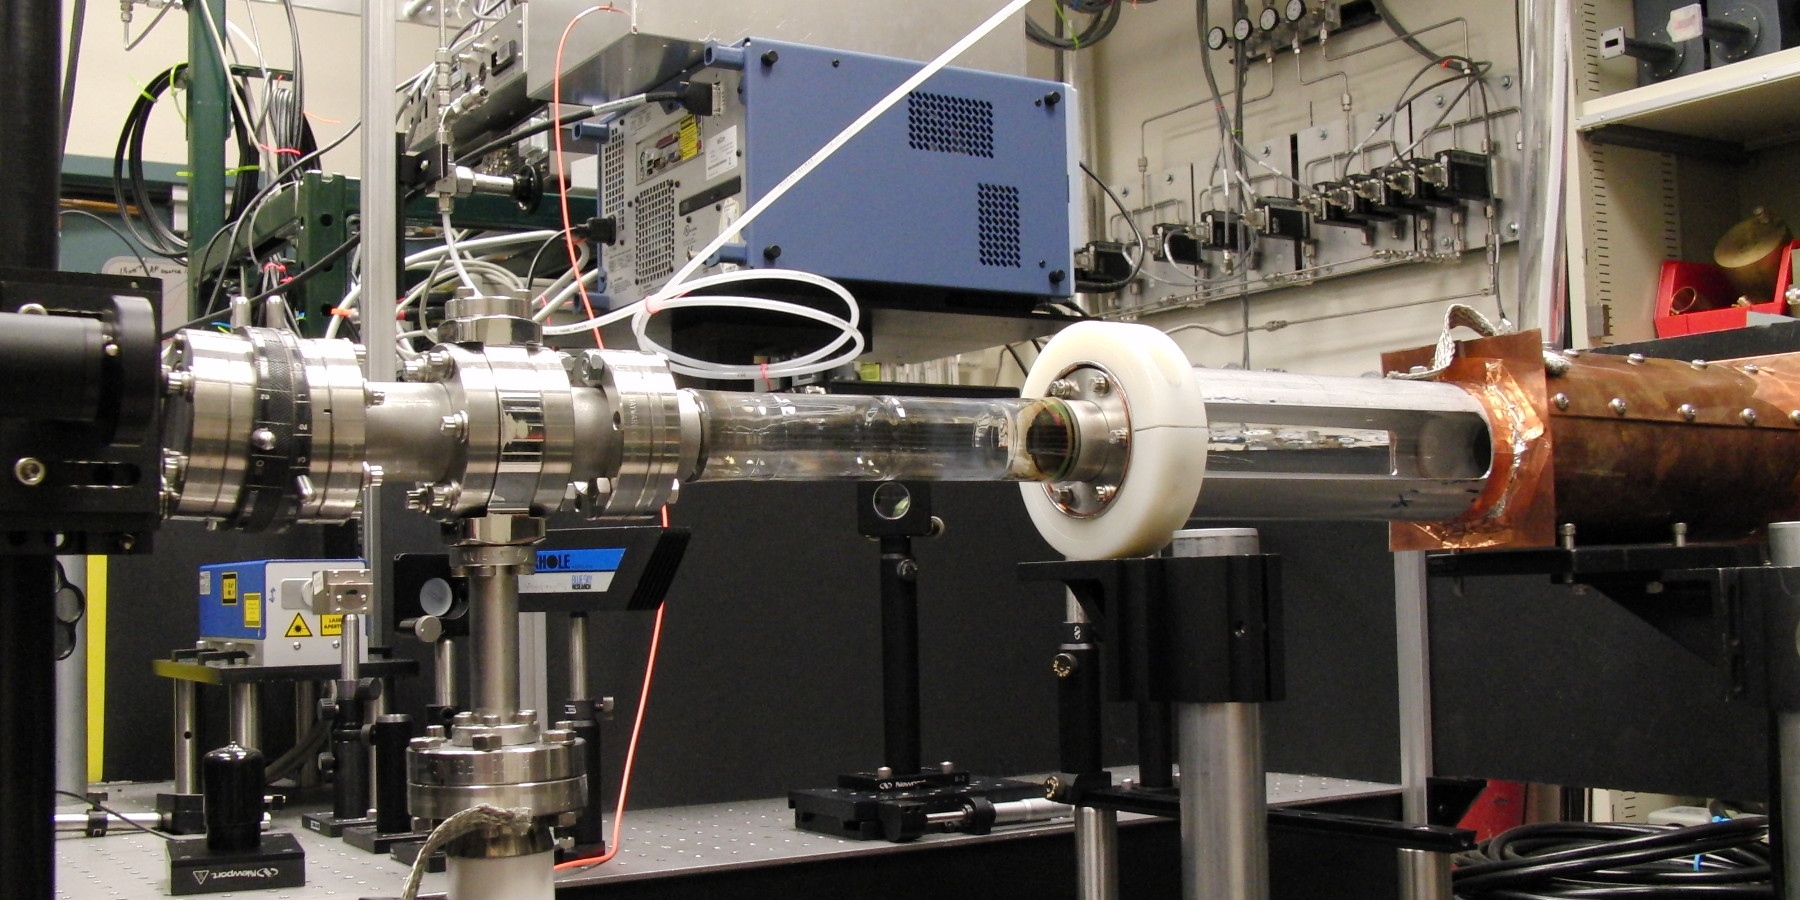
\includegraphics{./chapters/experiment/figures/appphoto.jpg}}
  \caption{Photograph of the discharge apparatus.}
  \label{fig:appphoto}
\end{figure}
The \acs{rpnd} apparatus was supported two 1.5 in mounting posts with angle
brackets. The mounting posts attached to a 4 ft by 2.5 ft optical breadboard,
supported by urethane shock absorbers, and a rigid frame. The roughing pump was
attached to the apparatus with flanged bellows in order to reduce vibrations. 

All electrical measurements were made with a LeCroy \smaller{6100A} WaveRunner
oscilloscope which had a bandwidth of 1.0 GHz. Electrical connections to the
oscilloscope were made with \smaller{RG 50/U} coaxial cable and standard
\textsc{bnc} connectors, terminated at 50 $\Omega$ unless otherwise noted. The
voltage of the pulses was monitored from $1:1000$ divider built into the power
supply. The current was measured from a current shunt located in a break of the
outer conductor of the transmission line. The current shunt was composed of 9,
low inductance, $1.0 \Omega$ resistors connected in parallel.
Figure~\ref{fig:bcs}
\begin{figure}
  \centering
  \setlength\fboxsep{0pt}
  \setlength\fboxrule{1.0pt}
  \fbox{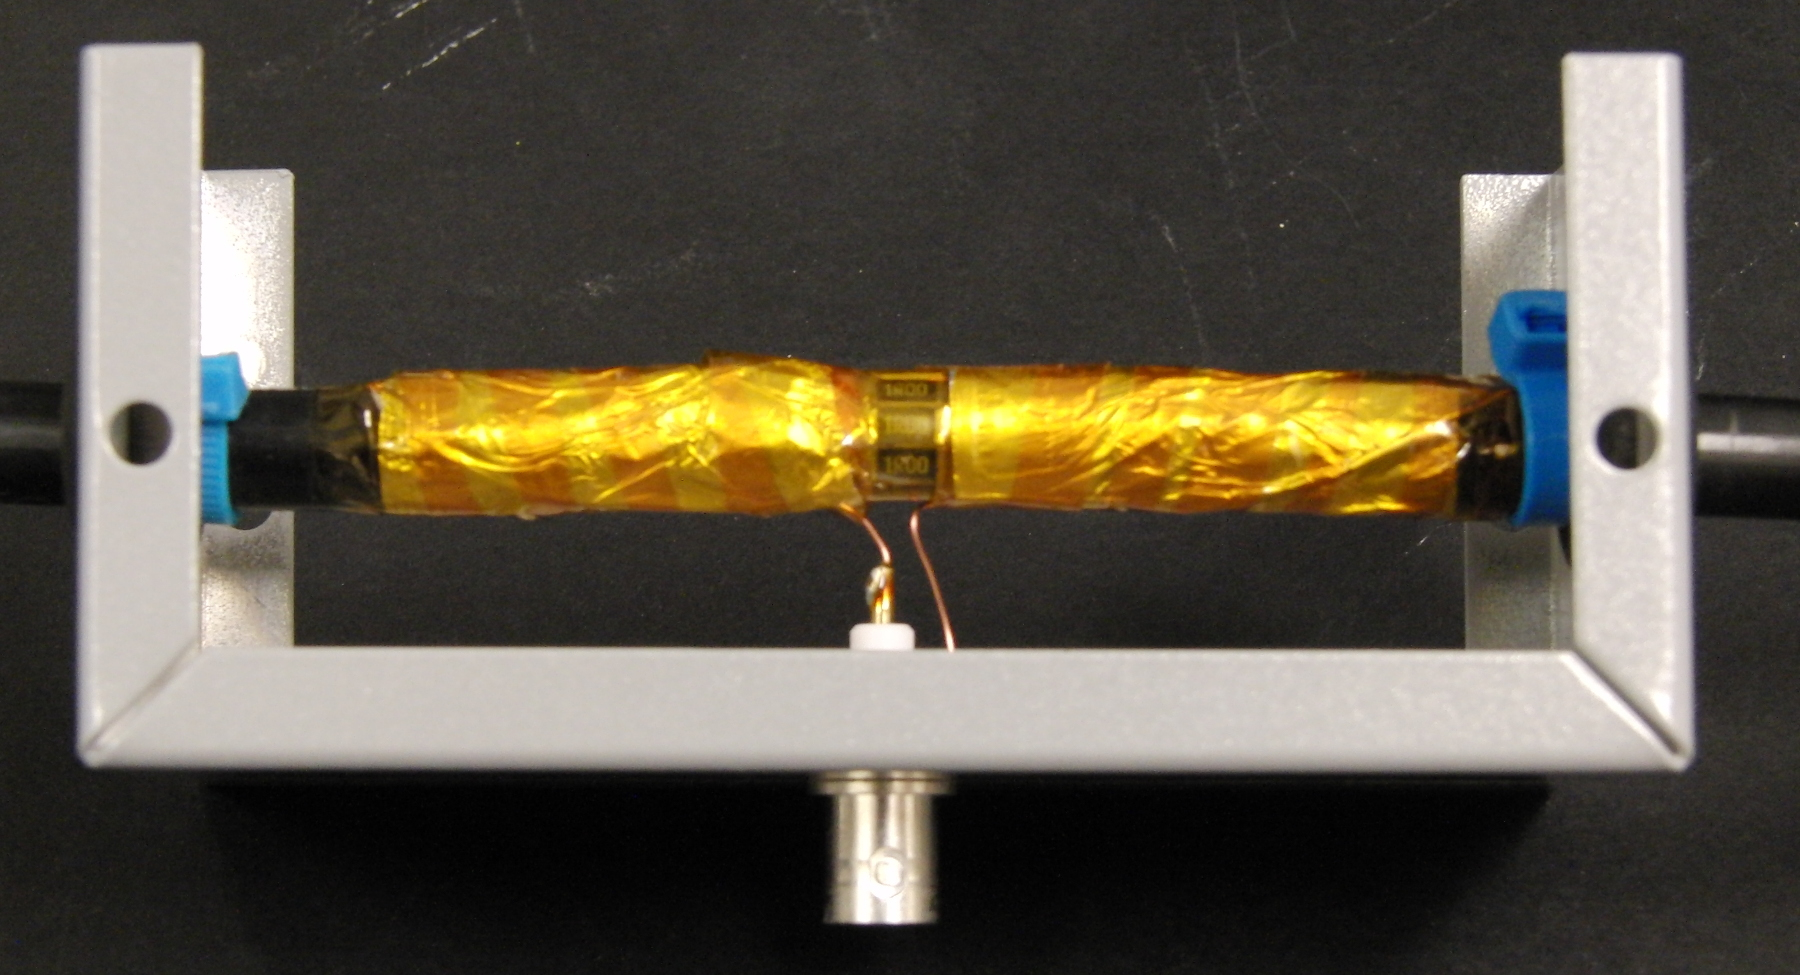
\includegraphics{./chapters/experiment/figures/bcs.jpg}}
  \caption{Photograph of the back-current shunt used to measure the current
  characteristics of the \acs{rpnd}.}
  \label{fig:bcs}
\end{figure}

Data were retrieved from the oscilloscope with a desktop computer via the
\textsc{gpib} interface. Instrument control, data acquisition, and data storage
were all managed by a LabView program. Analog input and output was handled with
the auxiliary input and output ports of a \textsc{srs} \smaller{SR850 DSP}
lock-in amplifier.

\section{Field Calculations}

The electric field characteristics of the discharge system was analyzed using a
two-dimensional, electrostatic solver, Ansoft Maxwell 9. Figure~\ref{fig:fields}
\begin{figure}
  \centering
  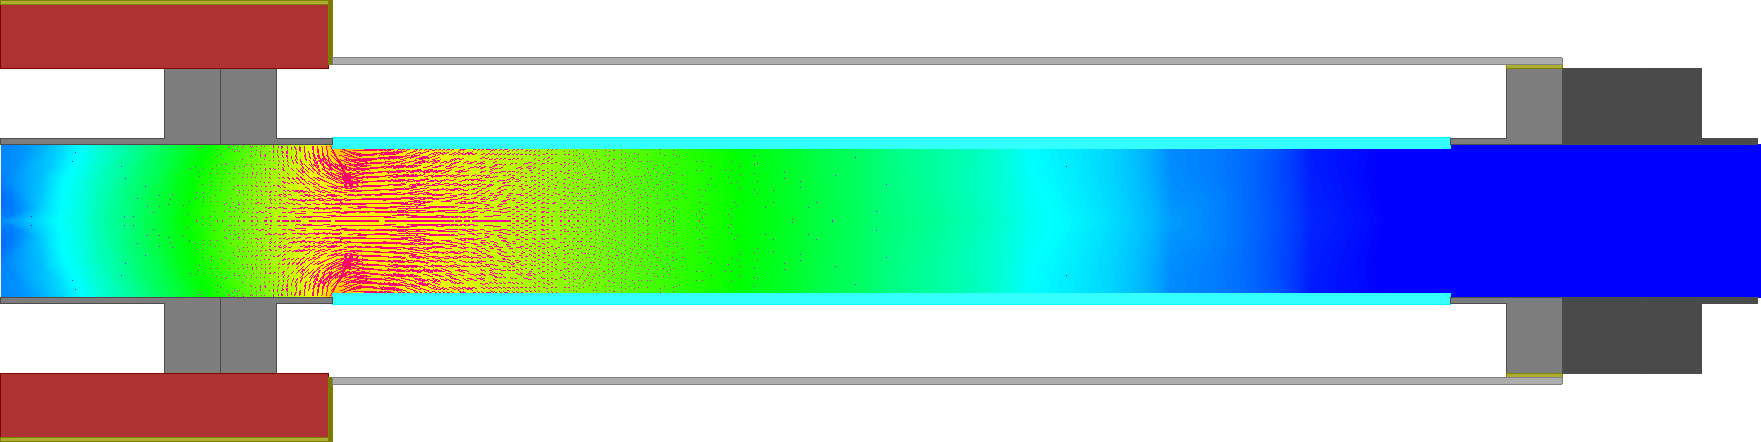
\includegraphics{./chapters/experiment/figures/fields.jpg}
  \caption{Heat map and vector plot of the electric field in the \acs{rpnd}
  discharge apparatus.}
  \label{fig:fields}
\end{figure}
is a heat map on a logarithmic scale, of the electric field magnitude, with
overlaid electric field vectors (in magenta). The electric field varies
significantly over the length of the discharge apparatus, with a peak near the
axial location of the glass tube followed by a monotonic decline. These
characteristics are a large departure from simple case of two parallel
electrodes in which the field is uniform throughout. This can be attributed to
the presence of the external ground shield. Though this does complicate the
field characteristics, the proximity of the ground results in a much higher
electric field than would otherwise be achievable.

While the off-axis field lines all feature notable radial components,
particularly close to the anode the center line does not.
Figure~\ref{fig:centere}
\begin{figure}
  \centering
  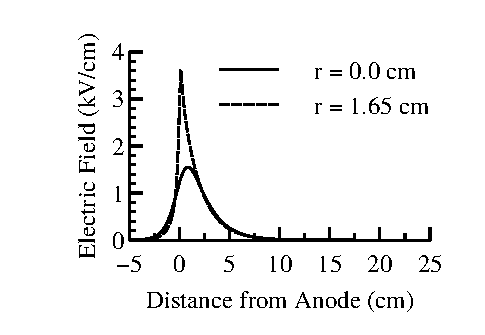
\includegraphics{./chapters/experiment/figures/centere.eps}
  \caption{The magnitude of the electric field along the center and outside of
  the discharge apparatus.}
  \label{fig:centere}
\end{figure}
is a plot of the magnitude of the electric field along the central axis of the
discharge apparatus and the outside, adjacent to the glass tube. The location of
the anode is defined as the location of the glass-to-metal seal. The field close
to the triple point at the seal is the highest at approximately 3.5 kV/cm, while
the field along the axis peaks at about 1.5 kV/cm. At a distance of 2 cm from
the anode, the electric field magnitude is roughly the same regardless of the
radial coordinate. At the measurement locations of 3.83, 11.45, and 19.07 cm,
the vacuum electric field was $4.8 \times 10^5$, 750, and 11 V/m respectively. 

\section{Operating Procedures}

One of two operating procedures was selected depending on how recently the
plasma had last been turned on. If it had been greater than one hour, a full
startup procedure was used. Otherwise, an abbreviated process was used. 

In order to obtain consistent discharge characteristics, it was necessary to
develop two sets of operating procedures for the \acs{rpnd}. In the case that
the discharge had not been operated for over an hour, the roughing pump was
turned on and the primary pump path valve was opened as was the first shutoff
valve upstream of the discharge chamber, seen in figure~\ref{fig:pump}.
\begin{figure}
  \centering
  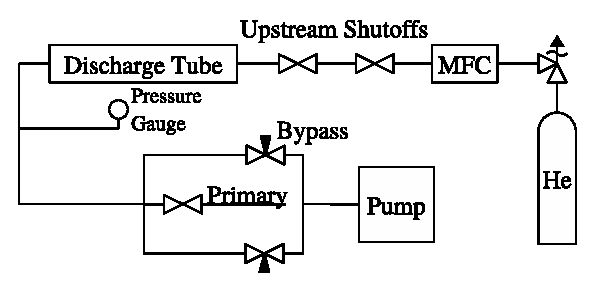
\includegraphics{./chapters/experiment/figures/pump.eps}
  \caption{Simplified diagram of the gas flow path and pumping system.}
  \label{fig:pump}
\end{figure}
The system was then allowed to pump down to its base pressure. Afterward the
final shutoff valve upstream of the pump path was opened and the system was
again allowed to reach base pressure. At this point the helium flow was turned
on and set to 25.0 sccm. The primary pump path was then closed and the needle
valve bypasses were used to adjust the system pressure to 3.0 Torr.

Next, the delay generator was turned on and the output for triggering the power
supply was activated. Then, the \acs{fid} power supply was then turned on. This
would produce an easily visible plasma within the discharge tube. The system was
allowed to operate at this condition for one hour in order to remove potential
contamination on the walls and electrodes. At the end of this period, the pulse
voltage waveform was checked to ensure that it was consistent with previous
waveforms. Once this was confirmed, the pressure was adjusted to the desired
operating condition.

The plasma was shutdown by first shutting off the power supply, followed by the
delay generator. Then, the helium flow was shut off, and the primary pump path
was opened. The system was allowed to come to base pressure before the two
upstream shutoff valves were closed, after which the primary pump path was
closed. The roughing pump was then shut off.

In the cases that the plasma had been operated within the last hour, it was
possible to use an abbreviated startup procedure. This process was fundamentally
the same as the previous one, however the plasma only required five minutes to
reach a steady state. This was verified with multiple measurements of the
current and voltage characteristics as well as the plasma emissions. At times
prior to this five minute equilibration period, the reflected pulse energy was
noticeably higher, and the delay between the trigger pulse and the output pulse
was variable.

\section{Electrical Characteristics}

The general voltage waveform of the \acs{rpnd} showed a number of
characteristics. Figure~\ref{fig:waveform}
\begin{figure}
  \centering
  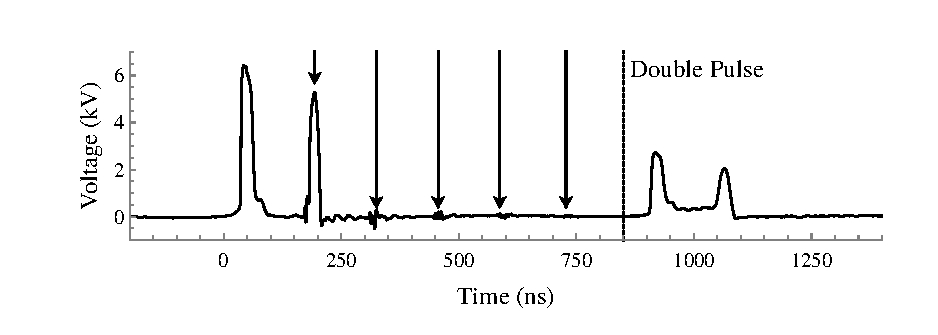
\includegraphics{./chapters/experiment/figures/waveform.eps}
  \caption{Typical voltage waveform of the \acs{rpnd}. Arrows indicate
    reflections back to the power supply. The dotted line delineates the time at
    which the power supply begins to exhibit double pulsing.}
  \label{fig:waveform}
\end{figure}
is a plot of a typical voltage waveform of the \acs{rpnd}. It begins with an
incident pulse with a small foot at $t = 0.0$. This followed by a reflected
pulse 138 ns afterward. The reflected pulse is somewhat attenuated, proportional
to the energy deposited in the plasma. Additional reflections are visible at
integer multiples of 138 ns, however they are highly attenuated. This suggests
that after the first pulse initiates the discharge, energy is much more easily
coupled into the volume. An additional pulse appears after about 800 ns. This is
believed to be a peculiarity of the power supply. For the most part, analysis of
the \acs{rpnd} will focus on the first 138 ns in order to isolate the effects of
a single pulse.

The independent variable for most operating conditions was the pressure of the
system. The properties of the \acs{rpnd} were examined at: 0.3, 0.5, 1.0, 2.0,
3.0, 4.0, 8.0, and 16.0 Torr. The appearance of the plasma varied with the
pressure in a continuous fashion, however it was apparent that there were three
regimes of operation.

At the low pressures, 0.3, 0.5, and 1.0 Torr, it was difficult to initiate the
discharge. Often, it would be necessary to increase the pressure to initiate the
discharge, and then reduce the pressure to the desired conditions. The plasma
appeared dim and relatively constricted to the central axis of the discharge
tube, with a radial extent of approximately 1 cm. Accompanying these presures
was a large degree of electronic noise. This manifested in the voltage and
current waveforms, seen in figure~\ref{fig:waveforms}, 
\begin{figure}
  \centering
  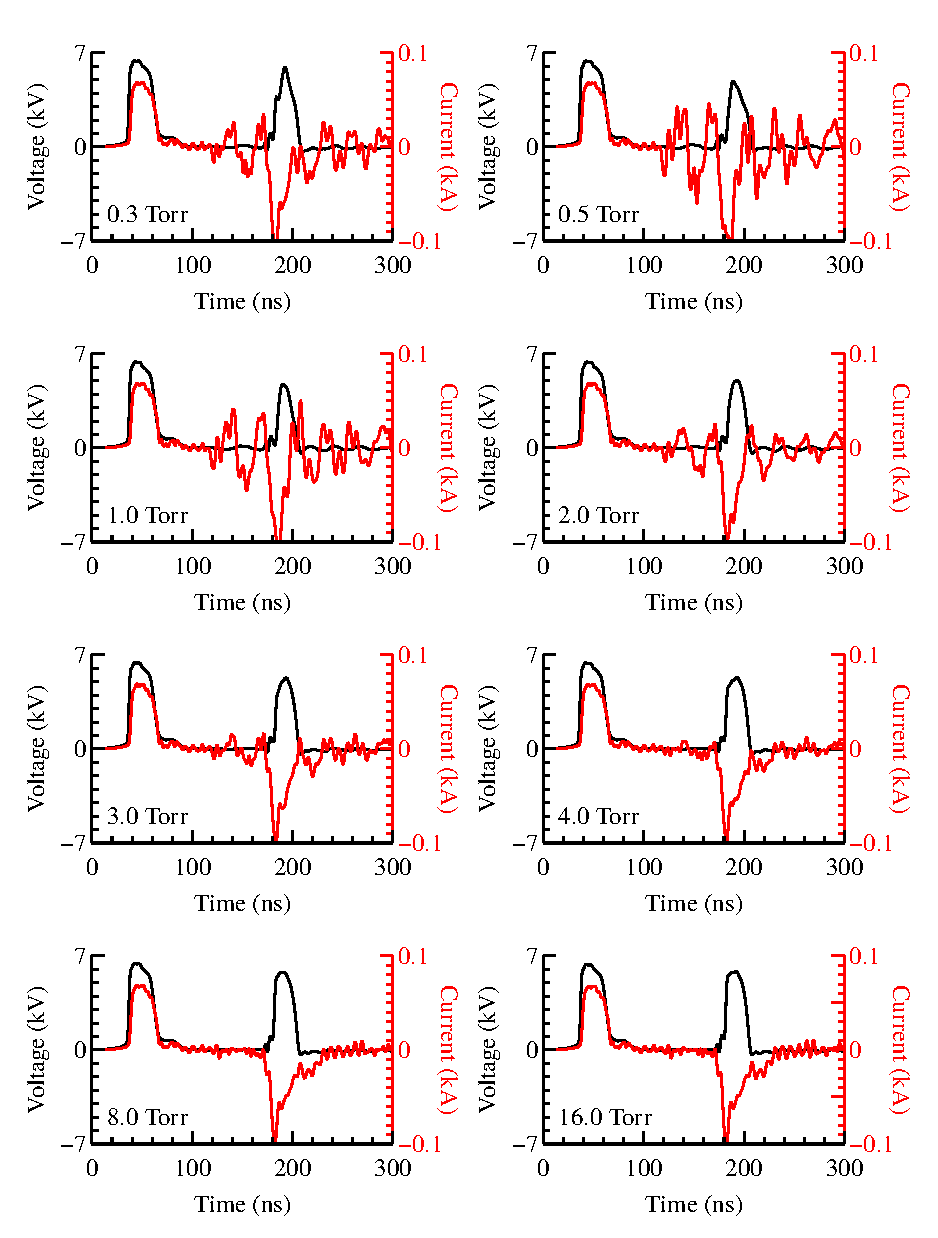
\includegraphics{./chapters/experiment/figures/waveforms.eps}
  \caption{High resolution views of the voltage and current waveforms for the
  first incident and reflected pulse, at each of the operating pressures.}
  \label{fig:waveforms}
\end{figure}
as well as a number of equipment malfunctions.

As the pressure was increased, the electrical noise began to subside. The
waveforms in figure~\ref{fig:waveforms} show significant reductions in the
ringing that was particularly prominent in the current waveforms. In addition,
the visual extent of the plasma increased substantially to the point where it
could be considered volume-filling. The plasma also increased its axial extent
as well, eventually reaching well past the cathode/ground. This was despite
attempts to isolate this portion of the apparatus from the plasma. It is
possible to attribute this to the relatively large surface area of the anode in
comparison to the cathode. If a sufficiently high electron current is being
drawn from the cathode, space charge could begin to limit further current
extraction.

However, the plasma receded back to the intended cathode structure at the higher
operating pressures, 8.0 and 16.0 Torr. This was accompanied by a decrease in
the apparent brightness of the plasma to levels similar to that of the low
pressure conditions. In contrast, the plasma appeared to remain volume-filling.
While discharge initiation was difficult at the higher pressures, it was not
accompanied by the electrical noise observed at lower pressures.

\section{Energy Coupling}

The energy coupling to the plasma for the first pulse was calculated by
integration of the current and voltage product for the first incident and
reflected pulse. Figure~\ref{fig:energy}
\begin{figure}
  \centering
  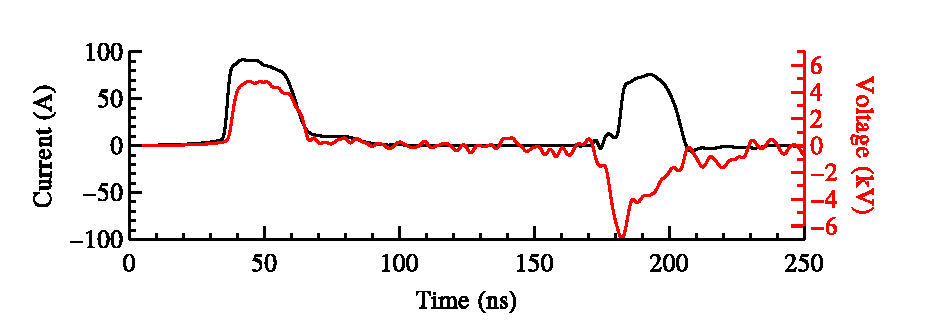
\includegraphics{./chapters/experiment/figures/energy.eps}
  \caption{Higher resolution plot of the initial voltage and current pulse.}
  \label{fig:energy}
\end{figure}
is a closer view of the time domain under consideration at the 4.0 Torr
condition. The voltage signal appears to be relatively unmarred by distortion or
ringing. The current signal from the shunt does appear to involve a moderate
degree of ringing. The ringing in the current signal increased at lower and
higher pressures and was most noticeable in the reflected pulse measurements.

Figure~\ref{fig:energies}
\begin{figure}
  \centering
  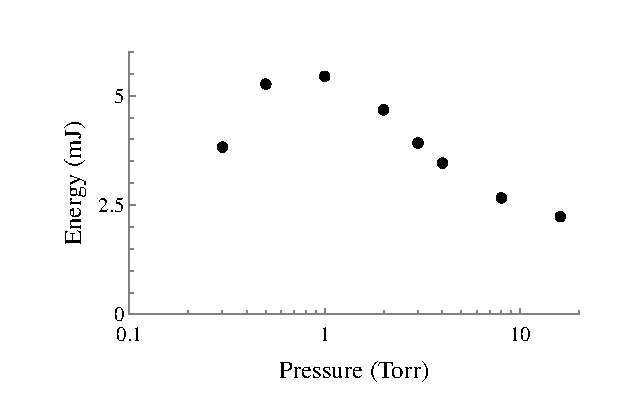
\includegraphics{./chapters/experiment/figures/energies.eps}
  \caption{Plot of the energy coupled into the plasma with the first pulse as
  a function of pressure.}
  \label{fig:energies}
\end{figure}
shows the energy coupled to the plasma for the first incident pulse as a result
of the above analysis. The coupled energy peaks at a pressure of 1.0 Torr and
5.5 mJ, before slowly decreasing. The uncertainty of these calculations is
difficult to estimate as error may be introduced by the ringing of the current
signal as well as timing differences between the current and voltage signals. 

There are no literature values for the energy coupling of a helium \acs{rpnd} to
compare to. However, several values exist for similar systems in other gases.
Nishihara et al.\ recorded energy coupling which ranged from 1-2 mJ in 250 Torr
of nitrogen \cite{Nishihara2006}. Pancheshnyi et al., in the study of an
air-propane mixture at 750 Torr, found that each pulse deposited about 1.9 mJ of
energy. Laroussi and Lu's study of a atmospheric-pressure helium plasma jet
estimated that the energy deposited per pulse was about 6-18 mJ based on the
power consumption of the power supply \cite{Laroussi2005}. Finally, Adamovich et
al.\ used semi-analytic solution to one-dimensional drift equations to estimate
the per pulse energy density in 40 Torr of air as 0.02-0.07 mJ/cm$^{-3}$
\cite{Adamovich2009}. The energy density for the results in
figure~\ref{fig:energies} ranged from about 0.01-0.02 mJ/cm$^{-3}$.
Interestingly, Adamovich et al.\ observe that the majority of the energy
deposition occurs in a very short time span after the initial breakdown of the
gas. A similar model by Nikandrov et al.\ produced similar results
\cite{Nikandrov2008}.
